\documentclass[thesis]{subfiles}

\begin{document}

\OnlyInSubfile{\appendix}
\chapter{Chemfiles: a library for chemistry input/output}
\label{sec:chemfiles}

During my PhD, I also wrote chemfiles, an open source library allowing to read
and write multiple file formats used in computational chemistry. I will present
here the software, its goals and some software architecture choices I made to
reach these goals. Chemfiles is available online at \url{https://chemfiles.org}
and \url{https://github.com/chemfiles}.

\vfill
\begin{figure}[H]
    \centering
    
\includegraphics[width=.3\textwidth]{figures/images/chemfiles-logo}
    \caption{Chemfiles' project logo}
    \label{fig:chemfiles:logo}
\end{figure}
\vfill

\newpage
\section{The computational chemistry formats zoo}

A recurrent pain point for anyone working in the theoretical and computational
chemistry field is the multiplication of file formats. Every simulation software
comes with its own set of files formats. And it is up to the user to adapt, and
learn how to work with the set of formats used by specific software. These
formats are used to store data generated by simulation software, before
analyzing it either through visualization of the atoms and their individual
motions; or by computing properties of the system from the positions and
velocities, using the framework of statistical thermodynamics presented in
section~\ref{sec:statistical-thermo}.

At the same time, every format contains the same kind of information: atomic
names, positions, velocities, forces, and topological information (bonds,
residues, \etc). Different formats exist because, in addition to storing these
basic data, they have different use cases. For example, the XYZ format is very
simple to read an write, both by hand and when creating new software. Binary
formats, such as NetCDF or TNG are able to store huge trajectories efficiently,
both in term of disk size and reading speed. The PBD, mmCIF and MMTF format are
optimized to store proteins and other bio-molecules.

\begin{figure}[ht]
    \centering
    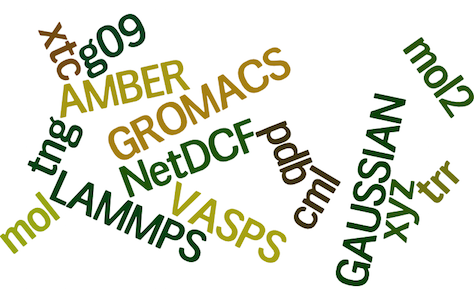
\includegraphics[width=.4\textwidth]{figures/images/files-formats}
    \caption{Some of the existing formats used in computational chemistry.}
    \label{fig:chemfiles:formats}
\end{figure}

This multiplication of formats means that there is less interoperability between
the different software used in computational chemistry. Analysis and
visualization software each support specific formats, which are not always the
same as the ones produced by simulation software. To run specific analysis on
the results of a simulation we have to either use readily available algorithms,
or learn how to read the format of our current software, and implement the
analysis ourselves. This friction can prevent switching between simulation
software or using specific analysis methods, and gets in the way of using the
tools of molecular simulation to improve our understanding of the world.

Chemfiles is an attempt to provide an unified and simple interface for
programmers to work with all these file formats. In order to do so, it defines a
representation for the data that can exist in various formats, and transparently
reads and writes files from and to this representation. Which means that
software developers only need to learn how to use chemfiles, and can then use it
to read or write every supported file format. Chemfiles is a software library; a
collection of functions and classes meant to be integrated into other software.
It can be used in simulation software (for example Domino uses chemfiles for
reading the initial configuration and writing the trajectory); visualization or
analysis software.

\newpage
\section{An overview of chemfiles}

\subsection{Goals and non-goals}

The main goal of chemfiles is to be useful to the research community at large.
To be useful, chemfiles must first be usable, and different researchers and
software developers work with different computing environments. Chemfiles is
portable between different platforms, operating systems (Windows, GNU/Linux,
macOS), word sizes (32 or 64-bits environments) and CPU architecture (Intel,
ARM, PowerPC, \dots). It is also usable from multiple languages, to allow any
computation chemistry project to use it, regardless of the implementation
language the authors choose. The core of the library is written in \cxx, and it
offers interfaces to C, Python, Fortran, Julia, and Rust.

Computational chemistry is used with a wide range of systems, and each kind of
system has specific requirements, which chemfiles tries to support. For
example, simulations of bio-molecules such as proteins or nucleic acid strands
use complex topologies, grouping some atoms in residues or monomers.
Oftentimes, this topology is stored in a separated file. While bio-molecules
simulation mostly only needs orthorhombic unit cells, material science and
crystallographic data need to describe triclinic unit cells, where some of the
angles are not 90°. Finally, when working with simulations in the grand
canonical ensemble such as GCMC, the number of atoms in the system changes along
the trajectory. Support for such simulations where the number of atoms is not
constant is often missing from existing software.

Chemfiles also has explicit non-goals: features that should not be part of
chemfiles itself, but could instead be built on the top of it. For example,
trajectory analysis, energy minimization or simulation algorithms would add too
much complexity to the code. Chemfiles is also actively trying \textbf{not} to
create a new format. Instead, it focuses on providing interoperability between
existing formats.

\subsection{Existing alternatives}

% Multiple attempts to solve the issue of file format multiplication already
% exist. Here, I will review some of these, and compare them to chemfiles,
% given the goals stated above for this kind of library.

\subsubsection{OpenBabel}

OpenBabel\cite{OBoyle2011} is \cxx library that provides read and write
capabilities to other software. It is a well-established software supporting
more than 110 different file formats. Unfortunately, it only supports text-based
formats, and no binary formats such as Amber NetCDF or Gromacs TNG. Such binary
formats are used to store big trajectories, are faster and take less space than
equivalent text formats.

Two other caveats of OpenBabel for me were the complexity of the programming
interface, and its license. OpenBabel is distributed under the Gnu Public
License version 2 (GPL-v2), which requires any project using it to be released
under the same license. This is due to the project's history, which was created
from the OELib project, itself distributed under the GPL license. This
requirement makes it harder to use OpenBabel in projects which use another
license, either another open source license or proprietary software developed by
a private company.

Concerning the programming interface, OpenBabel is written with the \cxx 98
standard, and a lot of member functions return raw pointers to internal data
directly, instead of the more modern references or smart pointers introduced
with \cxx11. This type of interface means that the programmer using the library
needs to manage memory manually, which in turn introduces more memory bugs in
the applications. Furthermore, I find the overall interface to be complex and
hard to learn, with many different functionalities not directly related to file
reading and writing. For example, it contains functions to search low energy
conformers, to create graphical images of molecules or to manage chemical
reactions. All of these functionalities are useful for cheminformatics
applications, but can clutter other uses of OpenBabel.

\subsubsection{Other alternatives}

\begin{table}[ht]
    \centering
    \caption{Summary of existing popular software library providing read/write
    capabilities for chemistry file formats.}
    \label{tab:chemfiles:alternatives}
    \def\nope{\textcolor{red}{✗}}
    \def\yep{\textcolor{webgreen}{✓}}
    \begin{tabularx}{0.8\textwidth}{X c c c c}
        \toprule
        \bfseries Project            & language & \cxx compatible & GCMC  & license \\
        \midrule
        OpenBabel\cite{OBoyle2011}   &   \cxx   &      \yep       & \nope & GPL-2   \\
        VMD\cite{Humphrey1996}       &  C/\cxx  &      \yep       & \nope & BSD     \\
        MDAnalysis\cite{Michaud2011} &  Python  &      \nope      & \nope & GPL-2   \\
        cclib\cite{OBoyle2008}       &  Python  &      \nope      & \nope & BSD     \\
        ASE\cite{HjorthLarsen2017}   &  Python  &      \nope      & \nope & LGPL    \\
        CDK\cite{Willighagen2017}    &  Java    &      \nope      & \nope & LGPL    \\
        \bottomrule
    \end{tabularx}
\end{table}

Multiple other alternatives to OpenBabel also exist, with different set of
goals and implementations; I summarize the most popular ones in
table~\ref{tab:chemfiles:alternatives}. Unfortunately, none of these
alternatives support GCMC simulations, with a number of molecules which can vary
during the simulation. Other than OpenBabel, only VMD molfile plugins (written
in C and \cxx) are compatible with \cxx simulation software.

I could not find an existing library that would cover all of my needs, which is
why I started working on chemfiles. I hope to increase the number of options
available to developers of chemical scientific software, and provide tools for
users of these software improving interoperability. Chemfiles is open source,
distributed under the BSD license at
\url{https://github.com/chemfiles/chemfiles}. This license roughly means that
anyone can download, use, modify and distribute the code --- even together with
software released under different licenses --- if they provide attribution of
the code to the original authors.

\subsection{Some code statistics}

I started working on chemfiles in December 2014, and released the version 0.1
the 16th of May 2015. Since then, I released 8 new versions, the last one being
version 0.9, which was released on the 31 of March 2019. During this period,
they have been 1500 git commits (self-contained modifications) in the core \cxx
chemfiles library, leading to a library containing 23 000 lines of code, as well
as 11 000 lines of test code. Bindings to chemfiles in other languages (Python,
Fortran, Rust, Julia) collectively contains 800 commits, 12 000 lines of code,
and 5 000 lines of tests.

A few people helped me making chemfiles what it is today, I would like to thank
them all here again: Jonathan Fine from Purdue University (USA); Patricio Germán
Barletta from Universidad Nacional de Quilmes (Argentina); Laura Scalfi and Elsa
Perrin from École Normale Supérieure (France).

\newpage
\section{Architecture and functionalities}

In this section, I will describe the general architecture of chemfiles, and then
dive into some specific features which I believe to be interesting in this
context. In particular, I will describe how one can store additional metadata in
a statically compiled language; the implementation and specificities of chemfiles'
atomic selection language; and how to use a software library from multiple
different programming languages.

\subsection{Public classes}

The full interface to chemfiles is contained into eight public classes, which
are represented in figure~\ref{fig:chemfiles:classes}. The starting point is the
\texttt{Trajectory} class, which provides functions to read or write a
\texttt{Frame}, as well as managing metadata associated with the trajectory. The
\texttt{Trajectory} does not do the actual work of parsing and formatting data,
which is delegated to the \texttt{Format} classes, presented in
section~\ref{sec:chemfiles:formats}.

\begin{figure}[ht]
    \centering
    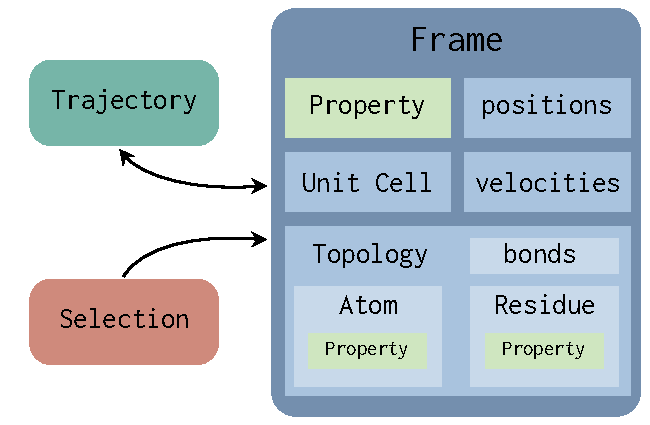
\includegraphics[width=0.6\textwidth]{figures/images/chemfiles-classes}
    \caption{Relation between chemfiles' public classes.}
    \label{fig:chemfiles:classes}
\end{figure}

The \texttt{Frame} class is the central class of chemfiles, it stores all the
data associated with a simulation step: positions, velocities, \texttt{UnitCell}
and \texttt{Topology}, and various properties. The \texttt{UnitCell} class
describes the unit cell of the simulation, and provides calculation of distances
that accounts for periodic boundary conditions. The \texttt{Topology} contains
the atoms and connectivity elements of the system: bonds, angles, dihedral
angles, and improper dihedral angles; but also residues. \texttt{Atoms} store
basic data associated with each atom: its name and type as character strings,
its mass and charge as floating point values. For some formats, the atomic name
and type are different: the atomic type will identify an atom or an extended
particle ("He", "Ow", "CH4"); while the atomic name might be a unique
identifier of this specific atom ("C\_a1", "Ow22"). \texttt{Residue} stores
additional atomic grouping, such as molecules, amino- or nucleic-acids, \etc

The \texttt{Property} class can be associated with either a frame, an atom or a
residue. It stores additional metadata that only occurs in some specific
formats, such as atomic hybridization state, molecule name or chain identifier
in bio-molecules. Finally, the \texttt{Selection} class implements chemfiles'
atomic selection language, which can be used to get a list of atoms matching
some constraints, such as \texttt{name == O and x < 22} or \texttt{pairs:
name(\#1) O and name(\#2) F and is\_bonded(\#1, name C)}. I will describe this
functionality with more details in section~\ref{sec:chemfiles:selections}.

\subsection{Files and formats}
\label{sec:chemfiles:formats}

As mentioned above, chemfiles' trajectory does read or write frames by itself.
Instead, it uses a subclass of the \texttt{Format} pure virtual abstract base
class. Each supported format is a specialization of this base class,
implementing at least one of three operations: read the next step of the
trajectory, read an arbitrary step of the trajectory, or write a single frame to
the trajectory. Implemented formats as of the 0.9 version of chemfiles are
listed in table~\ref{tab:chemfiles:formats}.

\begin{table}[ht]
    \centering
    \caption{List of format supported by chemfiles as of the 0.9 release, with
    associated file extension, classification as text or binary format and
    read or write support.}
    \label{tab:chemfiles:formats}
    \def\nope{\textcolor{red}{✗}}
    \def\yep{\textcolor{webgreen}{✓}}
    \begin{tabular}{l l c c c}
        \toprule
        Format                         & extension & text based & can read & can write \\
        \midrule
        Amber NetCDF\cite{AmberNetCDF} & .nc       & \nope      &  \yep    & \yep   \\
        CSSR                           & .cssr     & \yep       &  \yep    & \yep   \\
        DCD                            & .dcd      & \nope      &  \yep    & \nope  \\
        GRO                            & .gro      & \yep       &  \yep    & \yep   \\
        LAMMPS Data                    &           & \yep       &  \yep    & \yep   \\
        LAMMPS                         &.lammpstrj & \yep       &  \yep    & \nope  \\
        mmCIF\cite{Bourne1997}         & .mmcif    & \yep       &  \yep    & \yep   \\
        MMTF\cite{Bradley2017}         & .mmtf     & \nope      &  \yep    & \yep   \\
        MOL2                           & .mol2     & \yep       &  \yep    & \yep   \\
        Molden                         & .molen    & \yep       &  \yep    & \nope  \\
        PDB\cite{Berman2003}           & .pdb      & \yep       &  \yep    & \yep   \\
        SDF                            & .sdf      & \yep       &  \yep    & \yep   \\
        TNG\cite{Lundborg2013}         & .tng      & \nope      &  \yep    & \nope  \\
        TRJ                            & .trj      & \nope      &  \yep    & \nope  \\
        TRR                            & .trr      & \nope      &  \yep    & \nope  \\
        Tinker                         & .arc      & \yep       &  \yep    & \yep   \\
        XTC                            & .xtc      & \nope      &  \yep    &\nope   \\
        XYZ                            & .xyz      & \yep       &  \yep    & \yep   \\
        \bottomrule
    \end{tabular}
\end{table}

There are two main types of formats: text-based formats store data in a text
file, which must be parsed to extract the data. Some notable examples of
text-based formats include the XYZ, PDB and CIF formats. In all text formats,
floating point data such as positions will be stored as the list of characters
representing their digits in base 10, which must be parsed to reconstruct the
data.

The other class of formats is binary formats, including Amber NetCDF,
GROMACS TNG or XTC. In these formats, data is directly stored as a set of bytes
in the file, which can directly be interpreted as the corresponding floating
point type without additional transformations (except for managing the order in
which bits are written inside a byte, also called \emph{endianess}). Using a
binary format allows to use less space to store the same data: for example the
number 1.23456789 requires 10 bytes when represented as text using UTF-8
encoding, and only 4 as single precision IEEE-754 floating point number. Some
formats such as XTC uses additional molecular simulation specific encoding (such
as reduced decimal precision up to \SI{e-3}{\AA}) to reduce storage size even
further. This is particularly important for long simulations of large systems,
where the trajectory size can easily grow to multiple hundreds of gigabytes. All
these features combine to make binary formats more space- and time-efficient
than text-based formats: I found Amber NetCDF trajectories to take roughly five
times less space than the corresponding XYZ file, and be five times faster to
read.

Most binary formats come with a C or \cxx software library that should be used
to read or write them, or use another generic binary format with conventions
specific to molecular simulations. This is the case of Amber NetCDF, using the
NetCDF format\cite{AmberNetCDF}, MMTF using the MessagePack
format\cite{Bradley2017}, or H5MD using HDF5 data storage\cite{DeBuyl2014}.
This is their main shortcoming when compared to text-based formats, which does
not require special software to create or edit a file: any text editor can be
used.

In chemfiles, the file being read or written is managed by a subclass of either
the \texttt{TextFile} or \texttt{BinaryFile} classes. \texttt{BinaryFile} mainly
provide \cxx style memory management with constructors and destructors on the
top of the format library data structures. Text-based formats use
\texttt{TextFile} which works slightly differently: the base class defines an
interface (based on \cxx streams), which is then implemented by multiple child
classes. The formats can use any implementation to get access to the data. In
addition to the obvious basic file reader, chemfiles uses this to transparently
read and write compressed files with either the gzip (.gz files) or lzma (.xz
files) compression algorithms. All text-based format thus directly support
reading and writing compressed files without any specific code inside the format
class. In the future, this functionality could be expanded to transparently use
memory-mapped input/output which can be faster for some files; and to download
remote files from the internet.

\subsection{Storing additional data: properties}

Most formats store the same basic subset of data from a molecular simulation:
positions, velocities, atomic names, and connectivity. But they also store
additional data or metadata, which are specific to one or few file format. Being
able to read, store and possibly write back this data is important for two
reasons: it increases the amount of data that can be converted from one format
to another through chemfiles, assuming both format support storing it. Secondly,
it allows users of chemfiles working with a specific format to still access all
the data defined in the format.

Adding new attributes to atoms, frames or residues for every possible property
would not tractable. As most metadata are only defined by one or two
formats, adding a new data member in the classes would be a waste of memory. It
would also increase the complexity of the code, as implementing a new format
would require adding new data members not only to the core \cxx classes, but
also to the corresponding objects in the other languages bindings. Adding new
data member also means that it would be impossible to maintain a stable binary
interface between releases of chemfiles, as the size of classes would change.

Chemfiles solution is to introduce a dynamically typed property, which can be
attached to frames, atoms or residues in associative maps. The associative map
links each property with a property name, which can be used to check if the
property is defined on a given frame, atom or residue. The \texttt{Property}
class is a tagged union, containing a type tag which can change at run-time and
the associated data. It can contain either a character string, a Boolean value
(\emph{true} or \emph{false}), a number stored a double precision IEEE-754
floating point or a three-dimensional vector as three double precision floating
point numbers. These four types cover the vast majority of data found in
molecular simulation: for example, atomic forces can be stored as
three-dimensional vector atomic properties, and the user who created a
particular file can be stored as character string associated with the frame.
This strategy trades a small performance penalty at runtime --- the code must
check if a property exists, and if it has the right type -- for a huge
flexibility when storing additional data and metadata.

\subsection{Atomic selection language}
\label{sec:chemfiles:selections}
\newcommand{\token}[1]{\texttt{\bfseries#1}}

Chemfiles implements a rich selection language that allows finding the atoms in a
frame that match a set of constraints. For example, \texttt{atom: name == H and x
> 15} would select all atoms with a name equal to "H" and x cartesian coordinate
bigger than 15. Here, \texttt{name == H} and \texttt{x > 15} are individual
constraints, and they are combined with \texttt{and}, meaning both of them must
be true for an atom to match to full selection.

\subsubsection{Multi-atoms selections}

Chemfiles atomic selection language differs from other implementations such as
the one in VMD, MDAnalysis, or ASE (the Python Atomistic Simulation Environment)
by the fact that it is possible to formulate constraints not only on single
atoms, but also on pairs, triplets, and quadruplets of atoms. For example,
\texttt{angles: name(\#2) O and mass(\#3) < 1.5} will select all sets of three
bonded atoms forming an angle such that the name of the second atom is O and the
mass of the third atom is less than 1.5. Here, the first atom is left
unconstrained. Where evaluating simple selections yields a list of matching
atomic indexes, evaluating triplet selection will return a list of triplets of
atomic indexes (and correspondingly for pairs and quadruplets).

The number of atoms to select together is indicated in chemfiles by a context,
separated from the main selection by a colon. Seven contexts are available:
\token{atoms} is the default context, matching single atoms. \token{two},
\token{three}, and \token{four} match arbitrary pairs, triplets and quadruplets
respectively. \token{bonds}, \token{angles}, and \token{dihedrals} match pairs,
triplets and quadruplets of atoms bonded together to form the corresponding
connectivity element.

The selections are built by assembling simple constraints with Boolean operators:
\token{and}, \token{or} and \token{not}. They follow the usual interpretation of
logic: \texttt{A and B} will be true only if both A and B are true, \texttt{A or
B} will be true if one of A or B is, and \texttt{not A} will be true is A is
false. The constraints can check text values, such as \token{name} (atomic name),
\token{type} (atomic type), \token{resname} (residue name), with a fixed string
(\texttt{name(\#1) == Fe}) or another text value (\texttt{type(\#1) !=
type(\#3)}). There are also constraints on numeric values, for example \token{x},
\token{y}, \token{z} for the position of the atoms, \token{mass} for the atomic
mass, \token{index} for the index of the atom in the frame, \etc Numeric values
can be combined with the usual mathematical operations: \texttt{x\^{}2 + y\^{}2
+ z\^{}2 < 10\^{}2} will check for atoms inside the sphere with a radius of
\SI{10}{\AA} centered on the origin. Finally, Boolean constraints such as
\texttt{is\_bonded(i, j)}, \texttt{is\_angle(i, j, k)} or
\texttt{is\_dihedral(i, j, k, m)} are used to query the connectivity of atoms.
Here, the arguments to \texttt{is\_bonded} and the others can either be one of
the atoms currently being matched (\texttt{\#1}, \texttt{\#2}, \texttt{\#3},
\texttt{\#4}) or a sub-selection, and every atom matched by the sub-selection
will be checked. This makes for example \texttt{is\_bonded(\#1, name O)} select
all atoms bonded to an oxygen.

\subsubsection{Implementation strategy}

The transformation from a character string describing the constraints in a
domain specific language to a \texttt{Selection} object able to find the atoms
matching these constraints go through three main steps. First, the string is
transformed into a stream of simple tokens during an operation called
\emph{lexing}. For example, a single parenthesis \token{(} is a token, each
mathematical operator (\token{+}, \token{-}, \token{*}, \token{/},
\token{\textasciicircum}) is its own token, keywords such as \token{and} and
\token{or} are tokens, and single words such as \token{name} or \token{index}
are tokens.

Then, the tokens are checked for specific patterns during \emph{parsing}. For
example, if the tokens \token{name}, \token{==} and \token{"O"} are found in
this order, we know we have found a constraint stating that the atom name must be
equal to "O". Multiple different algorithms are available to implement the
parsing step, and chemfiles uses a recursive descent parser. This kind of parser
is built around multiple functions that can call each other (hence the
\emph{recursive} part of recursive descent), each function being able to parse a
small subset of the possible expressions. There is a function that recognize
additions and subtractions ($\cdots$ \token{+|-} $\cdots$), another one that
deals with multiplication and divisions ($\cdots$ \token{*|/} $\cdots$), \etc By
combining these function, it is then possible to parse complex expressions with
the right precedence. An example of recursive calling is the parsing of
\texttt{3 + 4 * (5 + 2)}. First the function for additions is called, and it
calls the one for multiplication to parse \texttt{4 * (5 + 2)}, which itself
calls the function for addition to parse \texttt{5 + 2}.

Finally, an \emph{Abstract Syntax Tree} (AST) is built from the recognized
constraints. Such tree is illustrated in figure~\ref{fig:chemfiles:selection-ast}
for the selection \texttt{name O and (x + y < 7 or index < 80)}. In this tree,
each node knows how to evaluate itself, by first asking its left and right
children to evaluate themselves and combining the results. AST in chemfiles deal
with three types of values: Boolean nodes create or combine Boolean values,
string nodes create character strings, and numeric nodes create or combine
numbers.

\begin{figure}[ht]
    \centering
    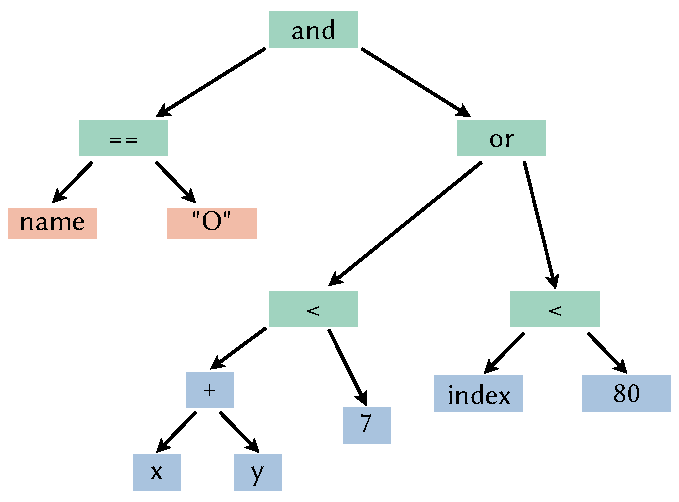
\includegraphics[width=0.6\textwidth]{figures/images/chemfiles-selection-ast}
    \caption{Abstract syntax tree for the selection \texttt{name O and (x + y <
    7 or index < 80)}. Nodes in green return a Boolean value, nodes in red a
    character string and nodes in blue deal with numbers.}
    \label{fig:chemfiles:selection-ast}
\end{figure}

To get the list of atoms matching the selection, the AST is walked from top to
bottom, evaluating individual components and combining them to build the full
answer to the question "does this set of atoms fulfill these constraints?".

\section*{Conclusions}

In this appendix, I presented chemfiles, an open source \cxx software library
that can be used to read and write a variety of file format produced by
computational chemistry software. Chemfiles currently supports 18 different
file formats, and I plan to add support for more popular formats, such as the
Crystallographic Interchange Format (CIF) and Protein Structure Files (PSF). It
also supports reading and writing compressed files for all text-based format.

The main goal of the chemfiles project is to produce a library simple enough
that scientist can learn it quickly and use it for their own needs. To do so, it
has a simple structure, with only seven public classes. Additional data and
metadata are represented as dynamically typed properties, keeping the overall
size of the programming interface small.

Chemfiles also features a rich and innovative atomic selection language, able to
use constraints on multiples atoms at once. While these selections are not
strictly central to file input and output, they are a central building block for
analysis and visualization software. The complexity associated with the
implementation and performance of selections justify their inclusion in a core,
shared library.

I used chemfiles in the \texttt{cfiles} command line tool to implement analysis
algorithms for molecular simulation. \texttt{cfiles} can compute radial
distribution functions; angles and dihedral angles distributions, density
profiles along a variety of axes (cartesian and radial) and density maps,
elastic constants from unit cell fluctuations in $NPT$
simulations\cite{Clavier2017}, hydrogen bonds and hydrogen bond autocorrelation,
and rotational autocorrelation. The autocorrelation of time series is computed
with a Fast Fourier Transform (FFT) approach, as the FFT algorithm is
$\mathcal{O}(n \log n)$ in the size of the input instead of $\mathcal{O}(n^2)$
for the naive version\cite{Kneller1995}. \texttt{cfiles} also provides some
tools to manage trajectory data, converting from a format to another and merging
multiple trajectories together.

\OnlyInSubfile{\printglobalbibliography}

\end{document}
